\documentclass[12pt, a4paper]{article}


\usepackage{hyperref}
\hypersetup{
    colorlinks,
    citecolor=blue,
    filecolor=blue,
    linkcolor=blue,
    urlcolor=blue
}

\usepackage{amsmath}
\DeclareMathOperator*\lowlim{\underline{lim}}
\DeclareMathOperator*\uplim{\overline{lim}}
% \usepackage{amsthm}
% \theoremstyle{definition}
\newtheorem{definition}{Definition}[subsection]
\newtheorem{theorem}{Theorem}[subsection]
\newtheorem{corollary}{Corollary}[subsection]
\newtheorem{exercise}{Exercise}
\usepackage{graphicx}
\usepackage{amsfonts}
\usepackage[letterpaper,margin=1in]{geometry}
\usepackage{float}
\usepackage{enumerate} 

\newtheorem{innercustomgeneric}{\customgenericname}
\providecommand{\customgenericname}{}
\newcommand{\newcustomtheorem}[2]{%
  \newenvironment{#1}[1]
  {%
   \renewcommand\customgenericname{#2}%
   \renewcommand\theinnercustomgeneric{##1}%
   \innercustomgeneric
  }
  {\endinnercustomgeneric}
}

\newcustomtheorem{customexercise}{Exercise}
\newcustomtheorem{customsol}{Solution}


\title{\textbf{Graph Rectifiability Summer Research with Lisa Naples} \\ [0.5cm] \sffamily{Daily Report}}

\author{\sffamily{By} \\[.2cm] \textbf{\textit{Charles Zhang}}  \\ [.5cm]}

\date{Summer 2021}

\begin{document}

\maketitle

\newpage
{
    \hypersetup{linkcolor=black}
    \tableofcontents
}

\newpage

\section{May 26}
\subsection{Exercises and Solutions}
\begin{customexercise}{1.12}
    Let $f, g:[0,1] \rightarrow \mathbb{R}$ be Lipschitz functions. 
    Show that the functions defined on $[0,1]$ by $f(x)+g(x)$ and 
    $f(x) g(x)$ are also Lipschitz.
\end{customexercise}

\textbf{Solution}:  
\begin{enumerate}[(i)]
    \item As $f, g$ are Lipschitz function, we have $|f(x)-f(y)| \leq c_1|x-y|$ and $|g(x)-g(y)| \leq c_2|x-y|$  where $\forall x, y \in [0, 1]$ and $c_1, c_2 \geq 0$.
    Then, $|(f(x)+g(x)) - (f(y) + g(y))| = |f(x) - f(y) +g(x) - g(y)| \leq  |f(x) - f(y)| + |g(x) - g(y)|\leq (c_1 + c_2 )\cdot |x - y|, \forall x, y\in[0, 1] $. Since $(c_1+c_2)\geq 0$, the condition is satisfied and therefore
    the functions defined on $[0,1]$ by $f(x)+g(x)$ is Lipschitz. 
    \item Consider that $|f(x) -f(0)| \leq c_1 |x| \leq c_1, x\in[0, 1]$, so we have non-negative $c_3 = |f(0)| + c_1 \geq |f(x)|$. Similarly, 
    we have non-negative $c_4 \geq |g(x)|$
    
    $|f|, |g| < 1$, $\forall x, y\in[0, 1]$\\
    $\begin{aligned}
        &|f(x)g(x) - f(y)g(y)| \\
        =& |f(x)g(x) -f(x)g(y) + f(x)g(y)- f(y)g(y)| \\
        =& |f(x)(g(x) - g(y)) + g(y)(f(x) - f(y))| \\ 
        \leq& |g(y)||(f(x) - f(y))| + |f(x)||(g(x) - g(y))| \\
        \leq& c_1 c_4 ||x-y| + c_2 c_3|x-y| \\
        \leq& (c_1c_4 +c_2c_3) |x-y|
    \end{aligned}$\\
    Since $c_1c_4 +c_2c_3 \geq 0$, the condition is satisfied and therefore
    the functions defined on $[0,1]$ by $f(x)g(x)$ is Lipschitz.
\end{enumerate}


\begin{customexercise}{1.13}
    Let $f: \mathbb{R} \rightarrow \mathbb{R}$ be differentiable 
    with $\left|f^{\prime}(x)\right| \leq c$ for all $x$. 
    Show, using the mean value theorem, that $f$ is a Lipschitz function.
\end{customexercise}

\textbf{Solution}: 
$\forall x, y \in \mathbf{R} , x \neq y$, by mean-value theorem, $\exists w \in(x, y)$ such that 
$$
\begin{aligned}
    &\frac{f(y)-f(x)}{y-x}=f^{\prime}(w) \\
    \Rightarrow  &\left|\frac{f(y)-f(x)}{y-x}\right|=\left|f^{\prime}(w)\right| \leq c \\
    \Rightarrow &|f(x)-f(y)| \leq c|x-y| \quad (x, y \in \mathbb{R})
\end{aligned}
$$

Therefore, $f$ is a Lipschitz function.


\begin{customexercise}{1.14}
    Show that every Lipschitz function 
    $f: \mathbb{R} \rightarrow \mathbb{R}$ is continuous.
\end{customexercise}

\textbf{Solution: } See proof wrote for Theorem \ref{LipschitzContinuous}.


\begin{customexercise}{1.15}
    Let $f: \mathbb{R} \rightarrow \mathbb{R}$ be given by $f(x)=x^{2}+x .$ 
    Find (i) $f^{-1}(2)$, (ii) $f^{-1}(-2)$ and (iii) $f^{-1}([2,6])$.
\end{customexercise}

\textbf{Solution}: As $f(x) = x^2 + x$, $\displaystyle x = -\frac{1}{2} \pm \frac{\sqrt{1 + 4y}}{2}$
\begin{enumerate}[(i)]
    \item $f^{-1}(2) = \{-2, 1\}$
    \item $f^{-1}(-2) = \emptyset$
    \item As $\displaystyle x = -\frac{1}{2} + \frac{\sqrt{1 + 4y}}{2}$ is increasing and $\displaystyle x = -\frac{1}{2} - \frac{\sqrt{1 + 4y}}{2}$ is decreasing while y increasing, 
     $f^{-1}([2,6]) = [-3, -2]\cup [1, 2]$
\end{enumerate}


\begin{customexercise}{1.16}
    Show that $f(x)=x^{2}$ is Lipschitz on $[0,2]$, bi-Lipschitz on 
    $[1,2]$ and not Lipschitz on $\mathbb{R}$.
\end{customexercise}

\textbf{Solution}: 
\begin{enumerate}[(i)]
    \item As $\forall x, y\in [0,2]$, $|x+y|\leq 4$, we have $|f(x)-f(y)|=\left|x^{2}-y^{2}\right|=|x+y||x-y| \leq 4|x-y|$.
    Thus, $f$ is Lipschitz on $[0,2]$.
    \item Apparently, $2|x-y|\leq|f(x) - f(y)|\leq 4|x-y|$ by above. As $f([1, 2]) = [1, 4]$, $\forall x, y \in [1, 4]$, $\displaystyle \frac{1}{\sqrt{x}+\sqrt{y}} \leq \frac{1}{2}$, we have: \\
    \(
    \begin{aligned}
        &\displaystyle \left|f^{-1}(x)-f^{-1}(y)\right|=|\sqrt{x}-\sqrt{y}|=\left|\frac{x-y}{\sqrt{x}+\sqrt{y}}\right| \leq \frac{1}{2}|x-y|\\
        \Rightarrow & \text{ so } f^{-1} \text{ is Lipschitz on } [1,4]. \\
        \Rightarrow & f \text{ is bi-Lipschitz on }[1,2].
    \end{aligned}
    \)
    \item Let $x = ky, k\in\mathbb{R}\setminus\{0\}$, then $\displaystyle \frac{|f(x) - f(y)|}{|x - y|} = \frac{|k^2y^2 - y^2|}{|ky - y|} = \left|\frac{k^2 - 1}{k-1} \right | |y|$, which is unbounded on $\mathbb{R}$. Therefore, the Lipschitz constant does not exist and $f$ is not Lipschitz on $\mathbb{R}$

\end{enumerate}


\newpage
\section{May 25}
\subsection{Basic Set Theory}

Review and summary of some definitions and theorems:

\begin{definition}[Countable]
    An infinite set $A$ is countable if its elements 
    can be listed in the form $x_1, x_2, ...$ with every 
    element of appearing at a specific place in the list; 
    otherwise, the set is uncountable
\end{definition}

\begin{definition}[Open]
    $A \subset \mathbb{R}^n$ is open if, $\forall x\in A$, $\exists B(x, r)\in A$ where $r>0$.
\end{definition}

\begin{definition}[Closed]
    $A \subset \mathbb{R}^n$ is closed if, whenever $\{x_k\}\in A$, $x_k\rightarrow x \in \mathbb{R}^n$, then $x\in A$.
\end{definition}

\begin{definition}[Closure]\label{closure}
    $\bar{A}$ is the intersection of all the closed sets containing a set A. 
\end{definition}

\begin{definition}[Interior]\label{interior}
    $int(A)$ is the union of all open sets contained in $A$.
\end{definition}

Definition \ref{closure} and \ref{interior} shows that The \textit{closure} 
of $A$ is thought of as the \textbf{smallest closed set} containing $A$, 
and the \textit{interior} as the \textbf{largest open set} contained in $A$.

\begin{definition}[Boundary]
    $\partial A = \bar{A}\setminus int(A)$
\end{definition}

\begin{theorem}
    $x\in\partial A \Leftrightarrow \forall r > 0, B(x, r) \cap A \neq \emptyset, B(x, r) \cap A^C \neq \emptyset$ 
\end{theorem}

\begin{definition}[Dense]
    Set $B$ is a dense in $A$ if $A\subset \bar{B}$, that is, if there are points of $B$ arbitrarily close to each point of $A$.
\end{definition}

\begin{definition}[Compact]
    $A$ is compact if any collection of open sets that covers $A$ has a finite subcollection which also covers $A$.
\end{definition}

\begin{theorem}
    A compact subset of $\mathbb{R}^n$ is both closed and bounded.
\end{theorem}

\begin{theorem}
    The intersection of any collection of compact sets is compact.
\end{theorem}

\begin{definition}[Connected]
    $A\subset \mathbb{R}^n$ is connected if there not exists open sets $U$ and $V$ s.t. $A\in U\cap V$ with disjoint and nonempty $A\cap U$ and $A\cap V$.
\end{definition}

\begin{definition}[Connected Component]
Connected component of $x$ is the largest connected subset of $A$ containing a point $x$.
\end{definition}

\begin{definition}[Disconnect]
    The set $A$ is totally disconnected if the connected component of each point consists of just that point.
\end{definition}

The definition of \textit{disconnect} also can be as: $\exists$ open sets $U$ and $V$ s.t. $x\in U, y\in V$ and $A\subset U\cap V$.

\begin{definition}[Borel Set]
    Borel Sets is the smallest collection fo subsets of $\mathbb{R}^n$ with the following properties:
    \begin{enumerate}
        \item Every open set and every closed set is a Borel set.
        \item The union of every finite or countable collection of Borel sets is a Borel set, and the intersection of every finite or countable collection of Borel sets is a Borel set.
    \end{enumerate}
\end{definition}

In short, Any set that can be constructed using a sequence of countable unions or intersections starting with the open sets or closed sets will certainly be Borel.

\subsection{Functions and Limits}

\begin{definition}[Congruence]
    The transformation $S : \mathbb{R}^n\rightarrow \mathbb{N}^n$ is congruence or isometry if it preserves distances i.e. if $|S(x)-S(y)| = |x-y|$ for $x, y\in \mathbb{R}^n$
    
\end{definition}

Special cases include \textit{translations}, which are of the form 
$S(x)=x+a$ and have the effect of shifting points parallel 
to the vector $a$, \textit{rotations} which have a centre $a$ such 
that $|S(x)-a|=|x-a|$ for all $x$ (for convenience, we also 
regard the identity transformation given by $I(x)=x$ as a 
rotation) and \textit{reflections}, which maps points to their mirror 
images in some $(n-1)$-dimensional plane. A congruence that 
may be achieved by a combination of a rotation and a translation, 
that is, does not involve reflection, is called a \textit{rigid motion} or 
\textit{direct congruence}. A transformation 
$S: \mathbb{R}^{n} \rightarrow \mathbb{R}^{n}$ is a \textit{similarity} of 
\textit{ratio} or \textit{scale} $c>0$ if $|S(x)-S(y)|=c|x-y|$ for all $x, y$ 
in $\mathbb{R}^{n} .$ A similarity transforms sets into geometrically 
similar ones with all lengths multiplied by the factor $c$.

\begin{definition}[Linear Transformation]
    A transformation $T : \mathbb{R}^n \rightarrow \mathbb{R}^n$ is linear 
    if $\forall x, y \in \mathbb{R}^n, T(x+y) = T(x) + T(y)$ and 
    $T(\lambda x) = \lambda T(x), \lambda \in\mathbb{R}$ 
\end{definition}

Such a linear transformation is \textit{non-singular} if $T(x)=0$ if and only if $x=0 .$ If 
$S: \mathbb{R}^{n} \rightarrow \mathbb{R}^{n}$ is of the form $S(x)=T(x)+a$, 
where $T$ is a non-singular linear transformation and $a$ is a vector in 
$\mathbb{R}^{n}$, then $S$ is called an \textit{affine transformation}\textit{ or an 
affinity}. An affinity may be thought of as a shearing transformation; 
its contracting or expanding effect need not be the same in every direction. 
However, if $T$ is orthonormal, then $s$ is a congruence, and if $T$ is a 
scalar multiple of an orthonormal transformation, then $T$ is a similarity.

\begin{definition}[Hölder Function]
    A function $f: X \rightarrow Y$ is called a Hölder function of exponent $\alpha$ if
$$
|f(x)-f(y)| \leq c|x-y|^{\alpha} \quad(x, y \in X)
$$
    for some constant $c\geq 0$.
\end{definition}

\begin{definition}[Libschitz Function]
    The function $f$ is called Lipschitz if
    $$
    |f(x)-f(y)| \leq c|x-y| \quad(x, y \in X)
    $$
    and bi-Lipschitz if 
    $$
    c_{1}|x-y| \leq |f(x)-f(y)| \leq c_{2}|x-y| \quad(x, y \in X)
    $$
    for $0<c_{1} \leq c_{2}<\infty$, in which case both $f$ and 
    $f^{-1}: f(X) \rightarrow X$ are Lipschitz functions.     
\end{definition}

\begin{definition}[Lower Limit]
    $$\displaystyle \lowlim_{x \to 0} f(x) \equiv \lim_{r\to 0}(inf\{f(x):0<x<r\})$$
\end{definition}

\textbf{Note:} $inf\{f(x):0<x<r\}$ is either $-\infty$ for all positive $r$ or else increases as $r$ decreases, 
$\lowlim_{x \to 0} f(x)$ always exists.

\begin{definition}[Upper Limit]
    $$\displaystyle \uplim_{x \to 0} f(x) \equiv  \lim_{r\to 0}(sup\{f(x):0<x<r\})$$
\end{definition}

\textbf{Note:} The lower and upper limits exist as real numbers or $-\infty$ or $\infty$ for 
every function $f$ and are indicative of the variation of $f$ for x close to 0, shown in Figure \ref{fig:lowerupperlimit}.

\begin{figure}[H]
    \centering
    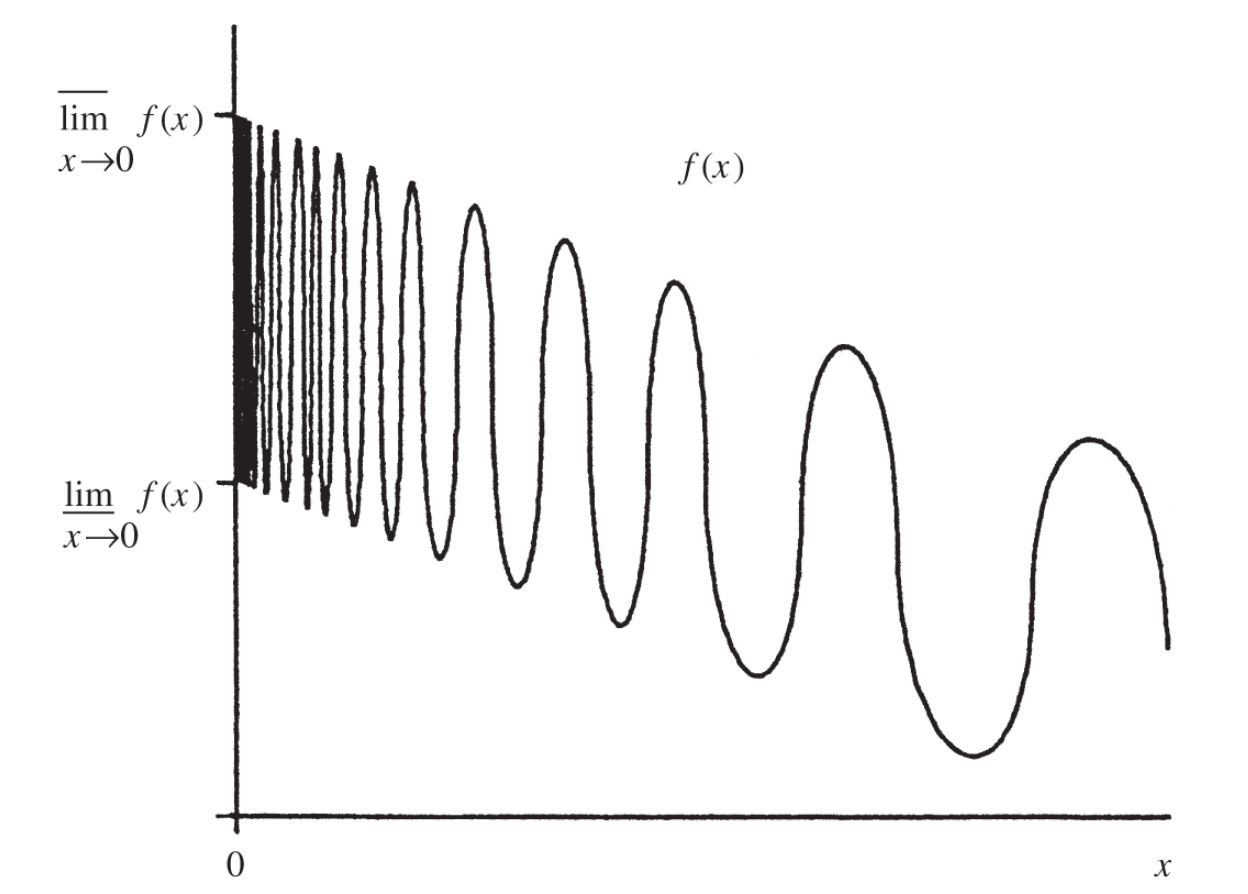
\includegraphics[width=.66\textwidth]{images/limit1.png}
    \caption{The upper and lower limits of a function.}
    \label{fig:lowerupperlimit}
\end{figure}

We write $f(x) \sim g(x)$ to mean that $f(x) / g(x) \rightarrow 1$ as $x \rightarrow 0$.

\begin{theorem}[Lipschitz functions are continuous]\label{LipschitzContinuous}
\end{theorem}

\textit{Proof}: Assum that the function $f: X \rightarrow Y$ is a Lipschitz function s.t. 
$|f(x)-f(y)| \leq c|x-y| (x, y \in X)$ for some constant $c\geq 0$.
Then, $\forall \epsilon > 0$, let $\displaystyle \delta = \frac{\epsilon}{c}$, and we have
$\forall x, y\in X, |x-y| < \delta \Rightarrow \displaystyle |x-y| < \frac{\epsilon}{c} \Rightarrow |f(x) - f(y)| \leq c |x-y| \leq c\cdot \frac{\epsilon}{c} = \epsilon \Rightarrow$ Lipschitz functions are continuous.

\begin{definition}[Homeomorphism]
    If $f: X \rightarrow Y$ is a continuous bijection with continuous 
    inverse $f^{-1}: Y \rightarrow X$, then $f$ is called a homeomorphism, 
    and $X$ and $Y$ are termed homeomorphic sets. 
\end{definition}
\begin{corollary}
    Congruences, similarities 
    and affine transformations on $\mathbb{R}^{n}$ are examples of homeomorphisms.
\end{corollary}

\begin{definition}[Differentiable]
    If $f: \mathbb{R}^{n} \rightarrow \mathbb{R}^{n}$, we say that $f$ is 
    differentiable at $x$ and has derivative given by the linear mapping 
    $f^{\prime}(x): \mathbb{R}^{n} \rightarrow \mathbb{R}^{n}$ if
$$
\lim _{h \rightarrow 0} \frac{\left|f(x+h)-f(x)-f^{\prime}(x) h\right|}{|h|}=0 .
$$
\end{definition}

\begin{definition}[Pointwise Convergence]
    For a sequence of functions: $f_k : X\rightarrow Y$ where $X$ and $Y$ are subsets 
    of Euclidean spaces. $f_k$ converge pointwise to a function $f:X\rightarrow Y$ if 
    $f_k(x)\rightarrow f(x)$ as $k\rightarrow \infty$.
\end{definition}

\begin{definition}[Unifrom Convergence]
    For a sequence of functions: $f_k : X\rightarrow Y$ where $X$ and $Y$ are subsets 
    of Euclidean spaces. $f_k$ converge uniformly to a function $f:X\rightarrow Y$ if 
    $sup_{x\in X} |f_k(x)- f(x)| \rightarrow 0$ as $k\rightarrow \infty$.
\end{definition}

\textbf{Note}: Uniform convergence is a stronger property than pointwise convergence i.e. Uniform convergence implies pointwise convergence, but not the other way around

\begin{theorem}
    If the functions $f_k$ are continuous and converge uniformly to $f$, then $f$ is continuous. 
\end{theorem}

\textit{proof:} TODO


\begin{theorem}[Logarithms]
    Apparently, $a^c = b^{c\log a / \log b}$
\end{theorem}
\end{document}